\setlength{\parskip}{1em}

\section{La explotación minera}
Una compañía minera requiere que le ayudemos a analizar su nueva explotación. Ha realizado el estudio de suelos de diferentes vetas y porciones del subsuelo. Con estos datos ha construido una regionalización del mismo. Cada región cuenta con un costo de procesamiento y una ganancia por extracción de materiales preciosos. En algunos casos el costo supera al beneficio. Al ser un procesamiento en profundidad, ciertas regiones requieren previamente procesar otras para acceder a ellas. \par

La compañía nos solicita que le ayudemos a maximizar su ganancia, determinando cuales son las regiones que tiene que trabajar. \par

\subsection{Solución}
%=============================================
Para modelar el problema, representaremos cada región como nodos. Cada nodo estará asociado tanto con las regiones que deberían ser explotadas previamente como con las que habilitaría la explotación de la región que este representa. Así, obtendremos un esquema idéntico al problema de "selección de proyectos" visto en clase. \par

A cada arista de esta red se le asigna un peso equivalente a la \textbf{cota de ganancia ${C+ 1}$} (suma de ganancias netas positivas más uno) y sentido hacia los nodos pre-requeridos.\par

Agregaremos entonces, para terminar de adaptar el modelo, un par de nodos sumidero y fuente, de cada lado del grafo. La fuente antecede a los que tengan ganancia neta positiva, y el sumidero sucede a las regiones con ganancia neta negativa. Cada arista de estos dos extremos que agregamos tendrá un peso o capacidad equivalente al módulo de la ganancia neta de su región asociada. Definimos \textbf{ganancia neta} como la diferencia entre la ganancia que ofrece una región y su costo.\par

A partir de este modelo, como se demostró en clase, el problema se reduce a obtener el corte mínimo del grafo obtenido. Para esto se implementa el \textbf{algoritmo de Ford-Fulkerson}, ya demostrado óptimo. Una vez obtenido este corte mínimo, podremos obtener el valor de la \textbf{ganancia máxima posible} ($G_{max}=C-CorteMinimo$) \textbf{y las regiones a explotar para conseguirla} (representadas por los nodos que quedan del lado de la fuente) \par


\newpage
\subsection{Pseudocódigo}

\begin{verbatim}
Llamar G al grafo que contiene a cada región y a cada región derivada
Llamar v_{i} a cada nodo que represente una región del grafo del problema
Llamar Gn_{i} a la ganancia neta de la región i
Llamar e_{i} a cada arista del grafo del problema, con peso Gn_{i}

Llamar C a la cota de ganancia neta (suma de ganancias netas positivas)
Llamar s al nodo fuente y t al nodo sumidero
Llamar Gmax a la ganancia máxima
    
Construir G, utilizando las regiones y los nodos s y t. 
Los nodos con Gn>=0 deben suceder a s y los Gn<0 anteceder a t.

Asignar a cada e_{i} que no conecte con s o t un peso equivalente a C + 1
Asignar a las restantes un peso equivalente a |Gn_{i}| .
    
Proceso FordFulkerson (G,C):
    corteMinimo = 0
    Gr = copia de G
    Mientras existe un camino de aumento p en Gr
        bn(p)::= capacidad mínima del camino p
        Para cada arista u->v en p
          disminuir la capacidad de u->v en bn(p)
          incrementar la capacidad de v->u en bn(p)
        fin para
        corteMinimo += bn(p)
    fin mientras
    En Gr, cada nodo alcanzable desde s es una región
a explotar (conjunto del corte mínimo de G).
    Gmax = C - corteMinimo

Sobre los caminos de aumento:
    Buscar un camino de aumento equivale a buscar un camino s->t 
(a través de aristas con capacidad no nula) usando DFS.
\end{verbatim}


\newpage
\subsection{Complejidad}
La complejidad temporal del algoritmo está dada por dos factores. La primera es la construcción del grafo que empleará el algoritmo de Ford-Fulkerson para resolver el problema de maximizar la ganancia.
Sea E la cantidad de aristas y sea V la cantidad de vertices. Luego, el coste de la construcción del grafo de $\mathcal{O}(E*V)$, siendo esta también su complejidad temporal.
Por otro lado, el algoritmo de Ford-Fulkerson, tiene una complejidad de $\mathcal{O}(V*q)$, donde $q$ es la cantidad de pasadas necesarias para hallar el corte mínimo y $V$ la cantidad de aristas. Se estima que el algoritmo tiene una probabilidad de requerir $n$ iteraciones de 1 en $4^n$.

\subsection{Ejemplo}
Supongamos que tenemos el siguiente caso:
\begin{center}
 \begin{tabular}{||c c c c c||} 
 \hline
 Región & Costo & Ganancia & Ganancia Neta & Prerequisitos \\ [0.5ex] 
 \hline\hline
 a & 10 & 5 & -5 & - \\ 
 \hline
 b & 15 & 5 & -10 & -\\
 \hline
 c & 25 & 5 & -20 & -\\
 \hline
 d & 5 & 15 & 10 & b, c \\
 \hline
 e & 5 & 20 & 15 & a\\ 
 \hline
 f & 10 & 30 & 20 & b\\ [1ex] 
 \hline
\end{tabular}
\end{center}
Las unidades son arbitrarias. Pueden representar miles o millones de pesos, por ejemplo. La cota de ganancia es 45 ($10+15+20$ por d, e y f). El grafo G entonces será:
    \begin{center}
    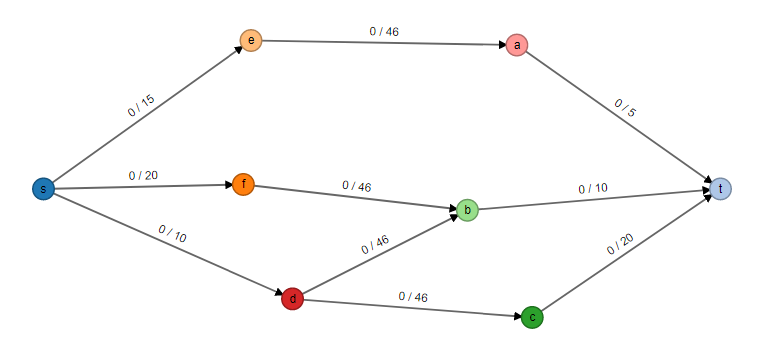
\includegraphics[width=0.9\textwidth]{Informe/Imagenes/Parte 2/ej1.png}
    \end{center}
Buscamos un primer camino de aumento. Este bien puede ser s-f-b-t. El cuello de botella en este camino es 10. Actualizamos las aristas de ese camino, disminuyendo la capacidad en 10 para el sentido original (color rojo) e incrementándola en 10 para el sentido inverso (color azul). Como en principio no tendremos aristas en los dos sentidos, las agregamos para todo el grafo. 
    \begin{center}
    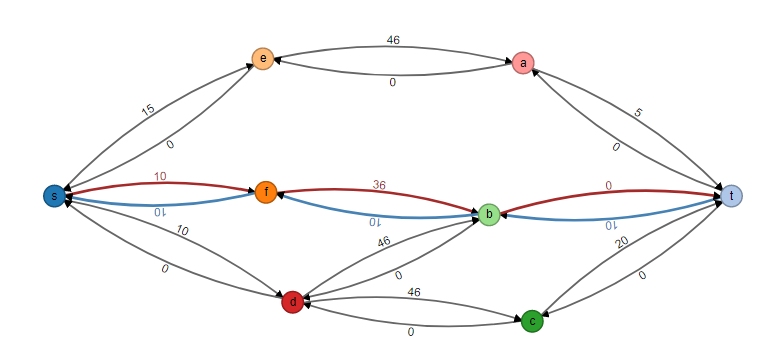
\includegraphics[width=0.8\textwidth]{Informe/Imagenes/Parte 2/ej2.png}
    \end{center}
El siguiente camino que tomamos es s-e-a-t. El valor mínimo acá es 5. Actualizamos las aristas.
\begin{center}
    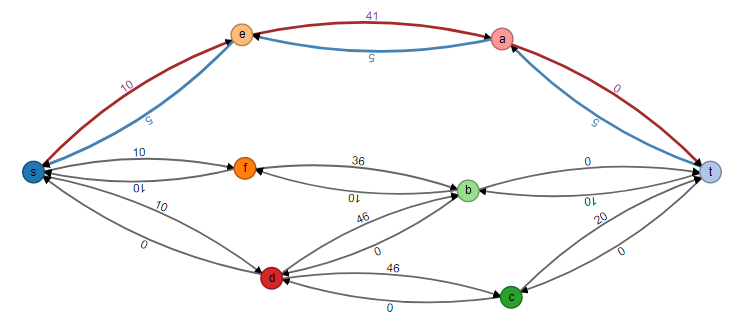
\includegraphics[width=0.8\textwidth]{Informe/Imagenes/Parte 2/ej3.png}
    \end{center}
Ahora tomamos el camino s-d-c-t, y su menor capacidad es 10. 
    \begin{center}
    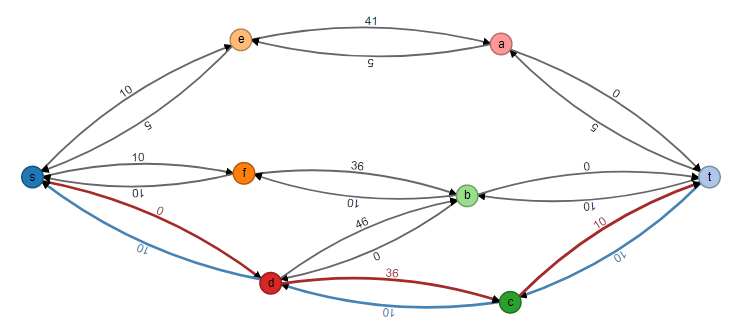
\includegraphics[width=0.8\textwidth]{Informe/Imagenes/Parte 2/ej4.png}
    \end{center}
Notar que la arista s->d quedó sin capacidad, por lo que no es más accesible desde s. Tampoco tenemos otro camino posible desde s hacia t, por lo tanto el algoritmo finalizó. Observando los nodos accesibles desde s, indicamos el corte mínimo con un trazo violeta. 
    \begin{center}
    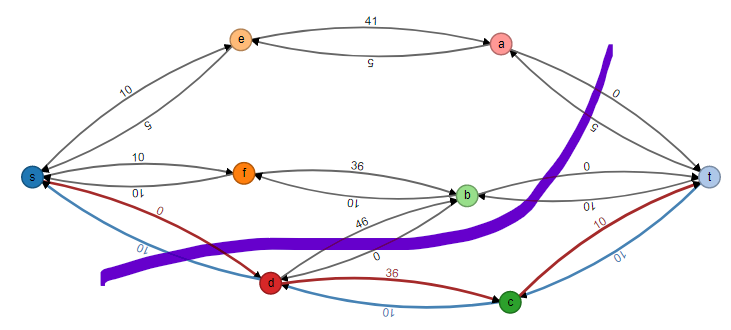
\includegraphics[width=0.9\textwidth]{Informe/Imagenes/Parte 2/ej5cm.png}
    \end{center}
Las regiones a explotar son las que se encuentran del lado s del corte:  \textbf{a, b, f y e}. Trazando el mismo corte en el grafo original, observamos que las capacidades de las aristas que van desde el lado s del corte hacia el lado t suman 25. Para conocer qué ganancia producirá esta explotación, queda restarle este valor a C; \textbf{la ganancia máxima será de 20}.
    \begin{center}
    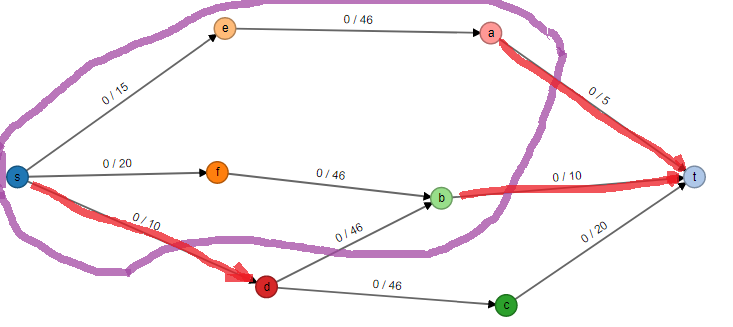
\includegraphics[width=0.9\textwidth]{Informe/Imagenes/Parte 2/ej6.png}
    \end{center}